The goal of this section is to illustrate in more detail the process a
system designer follows to add cyber requirements to the AGREE
specifications and then automatically transform the system to insert
the high-assurance components. The AGREE specifications generated by
the transforms for the high-assurance components are also
explained. The section ends with a concise formal statement of the
meaning of an AGREE specification for a high-assurance component. This
meaning is what must be preserved by the synthesis.

\newsavebox{\sw}
\begin{lrbox}{\sw}
\begin{lstlisting}[style=agree]
eq req : bool = event(AutomationRequest);
eq avl : bool = event(AirVehicleLocation);
eq wp : bool = event(Waypoint);
eq rsp: bool = event(Start);
eq alrt : bool = event(Alert);

assume "Automation request is well-formed" :
    req => WELL_FORMED_AUTOMATION_REQUEST(AutomationRequest);
assume "Air vehicle location is well-formed" :
    avl => WELL_FORMED_WAYPOINT(AirVehicleLocation);

eq current : bool = (req = rsp);
eq previous : bool = (req and not rsp) ->
                      pre(req and not rsp) and (not req and rsp);
eq policy : bool = current or previous;
eq since : bool =  alrt or (alrt and (false -> pre(since)));

guarantee "Start includes a waypoint" :
    rsp => wp;
guarantee "Locations required after the start waypoint" :
    (wp and not rsp) => avl;
guarantee "Waypoint is well-formed" :
    wp => WELL_FORMED_WAYPOINT(Waypoint);
guarantee "Alert if start is not bounded relative to a request" :
    policy or since;
\end{lstlisting}
\end{lrbox}

\begin{figure}
  \begin{center}
    \scalebox{0.60}{\usebox{\sw}}
  \end{center}
  \caption{The SW component contract.}
  \label{fig:sw}
\end{figure}

The AGREE specification for the SW component in the example of
Section~\ref{sec:example} with the added cyber requirements is given
in \figref{fig:sw}. The AGREE specification language is a first-order
predicate calculus that uses stream concepts, and operators, from the
Lustre language \cite{10.1145/41625.41641}. As with Lustre, the
semantics are synchronous dataflow where the inputs, outputs, and
expressions are data streams that comply with the input
assumptions. Contracts are evaluated in dependency order with inputs
being propagated to outputs through all contracts until they
stabilize; as such, the contracts, and thereby the top-level model,
must be acyclic.\footnote{An apparent syntactic cycle, where a
component is linked back to itself, may be broken temporally by
inserting delay elements.} Once the contracts have stabilized, the
model takes a synchronous step to the next input data in the
stream. The semantics do not model computation or communication
delay. The output of one contract is seen at the input of any
downstream contract in the same step of the input data stream.

The AGREE model checker attempts to prove several properties of the
top-level model being verified. The first is that the output
guarantees of each component implementing the system are strong enough
to validate the input assumptions of any downstream component as well
as to satisfy the guarantees of the output of the top-level component
being verified (\ie, the system composition meets input assumptions
at each input as well as the guarantees on the system output). These
properties are reported in the expanded lists
in \figref{fig:example}(b) and \figref{fig:hardened}(b).  The next set
of properties prove that the contract specifications for each
component are \emph{self-consistent} \ie, a contract does not contradict
itself. These are the unexpanded results at the bottom of the
figures.

Returning back to the contract of \figref{fig:sw}, it uses \texttt{eq}
statements to define variables local to the contract
specification. For example, the \texttt{req} variable is equivalent to
the \texttt{event(AutomationRequest)} expression. In the AGREE
semantics, there is an implicit \emph{event} input (or output)
associated with every named event port in a component. The semantics
used here do not buffer these events so the implicit input (or output)
is only a boolean value. An \texttt{event} expression refers to that
implicit input (or output) and is true when data is placed on the
named port. The system contract here states assumptions on well-formed
input, followed by guarantees on properties about the output.

The \emph{Alert if start is not bounded relative to a request}
guarantee is an invariant on the expression \texttt{policy or since},
meaning that either the policy holds or the alert is
sounding. The \texttt{policy} is defined by two local
values: \texttt{current} and \texttt{previous}. The \texttt{current}
value is asserted when in the current time step there is a request
with a response, or there is no request and no response.

The value of \texttt{previous} in the current time step relies on values from the previous time step. The \texttt{->} operator designates initialization, as the previous time step is undefined in the first step of the system. The left operand to the operator is the initial value of \texttt{previous} at start, which in this example is \texttt{(req and not rsp)}, because seeing a request with no response is inconclusive in the first step of the system. The right operand is the value of \texttt{previous} after the initial step. Here the \texttt{pre} operator refers to the value of the expression \texttt{(req and not rsp)} in the prior time step, \texttt{previous} is true if the previous time step made a request without a matching response and the current time step has the matching response to that request with no new request.

The value of \texttt{since} in \emph{Alert if start is not bounded relative to a request} relies on its own value in the previous time step. The intuitive reading of the expression is that the alert has been true since the time when it first sounded. The first \texttt{alrt} sets \texttt{since} to true, and once the value of \texttt{since} is true, that value persists as long as \texttt{alrt} holds. The \emph{Alert if start is not bounded relative to a request} guarantee defines one requirement of a cyber-hardened system implementation. Together with the other guarantees, the contract models the expected input and output of the system as a whole.

\begin{figure}
  \begin{center}
    \begin{tabular}{c}
      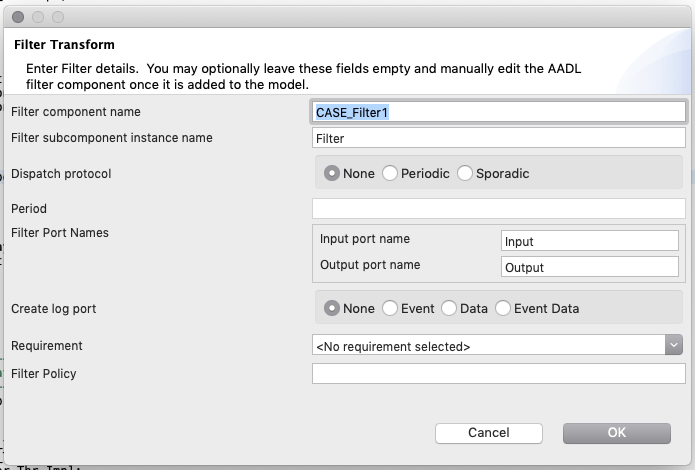
\includegraphics[scale=0.3]{dialogue.png}
    \end{tabular}
  \end{center}
  \caption{Wizard for automatically transforming the model with a filter.}
  \label{fig:dialogue}
\end{figure}

\newsavebox{\flt}
\begin{lrbox}{\flt}
\begin{lstlisting}[style=agree]
eq policy : bool =
  WELL_FORMED_AUTOMATION_RESPONSE(Input);
guarantee Filter_Output "Filter output is well-formed" :
  if event(Input) and policy then
    event(Output) and Output = Input
  else not event(Output);
\end{lstlisting}
\end{lrbox}

\newsavebox{\mntr}
\begin{lrbox}{\mntr}
\begin{lstlisting}[style=agree]
const is_latched : bool =
  Get_Property(this, CASE_Properties::Monitor_Latched);
eq rsp : bool = event(Response);
eq req : bool = event(Request);
eq current : bool = (req = rsp);
eq previous : bool = (req and not rsp) ->
                      pre(req and not rsp) and (not req and rsp);
eq policy : bool = current or previous;
eq alert : bool = (not policy)
                -> ((is_latched and pre(alert)) or not policy);
guarantee Monitor_Alert
  "Alert port tracks alert variable" :
  event(Alert) = alert;
guarantee Monitor_Output
  "Output if not alerted" :
  if event(Alert) then (not event(Output)) else
  if event(Response) then (event(Output) and (Output = Response))
  else (not event(Output));
\end{lstlisting}
\end{lrbox}

\begin{figure}
  \begin{center}
    \begin{tabular}{c}
      \scalebox{0.60}{\usebox{\flt}} \\
      (a) \\
      \scalebox{0.60}{\usebox{\mntr}} \\
      (b)
    \end{tabular}
  \end{center}
  \caption{High-assurance component contracts. (a) The filter. (b) The monitor.}
  \label{fig:assurance}
\end{figure}

As noted previously, the original system fails to guarantee the cyber requirements. BriefCASE provides two transformations to address the failing requirements: inserting a filter and inserting a monitor. The component is added by selecting the connection in the model where the high-assurance component is to be added, and then choosing the appropriate transformation. The system designer can provide transform configuration parameters in a wizard, as shown in \figref{fig:dialogue}. The policy of the high-assurance component can be stated directly in the wizard, or it can be left  blank. In this example, the policy is specified as \texttt{WELL\_FORMED\_AUTOMATION\_RESPONSE(Input)}.
Additionally, because a transformation is ultimately driven by a cyber requirement, BriefCASE updates an embedded Resolute assurance case~\cite{resolute-destion}.  Resolute keeps track of the evidential artifacts necessary for supporting the requirement, and can be run at any time to determine whether those artifacts are valid.
%Additionally, the filter can be attached to any requirement the vulnerability analysis. This association is useful the the assurance case from the Resolute tool [CITE DESTION 2021]. The \emph{OK} button creates the component and inserts it accordingly into the implementation

The AGREE contract specification generated by the transform is shown in \figref{fig:assurance}(a). The guarantee is stylized for synthesis and completely defines the meaning of the output under every possible input.
%A similar dialogue exist for inserting monitors that allows the system designer to add and remove inputs as needed.
The resulting AGREE specification for the monitor in this example is shown in \figref{fig:assurance}(b). The \texttt{is\_latched} value makes the alert persistent, meaning that once the alert is raised, it is always raised.  This behavior is one of the several options available in the dialogue. The definition for \texttt{policy} is taken by the system developer from the contract in \figref{fig:sw}. As before, the guarantees for the outputs are autogenerated by the tool and completely define each output under every possible input.
